\begin{figure}
  \usetikzlibrary{shapes.arrows, positioning}
  \definecolor{LightColor}{rgb}{1.0,0.901,0.805}
  \definecolor{EmptyColor}{HTML}{DCE2E6}

  \definecolor{tile0}{HTML}{DABDE4}
  \definecolor{tile1}{HTML}{B8DBF4}
  \definecolor{tile2}{HTML}{B5EDCD}
  \definecolor{tile3}{HTML}{FBEBA7}
  \definecolor{tile4}{HTML}{F9C1BB}
  \definecolor{tile5}{rgb}{1, 1, 1}

  \tikzstyle{array_element}=[rectangle,
                             minimum height=0.5cm, 
                             minimum width=0.5cm, 
                             minimum size=0.5cm,
                             draw=black,
                             rounded corners=2.5, ]
  \tikzstyle{empty_element}=[rectangle,
  fill=white
                                ]


  \begin{adjustbox}{minipage=\textwidth, scale=0.445}
    \centering
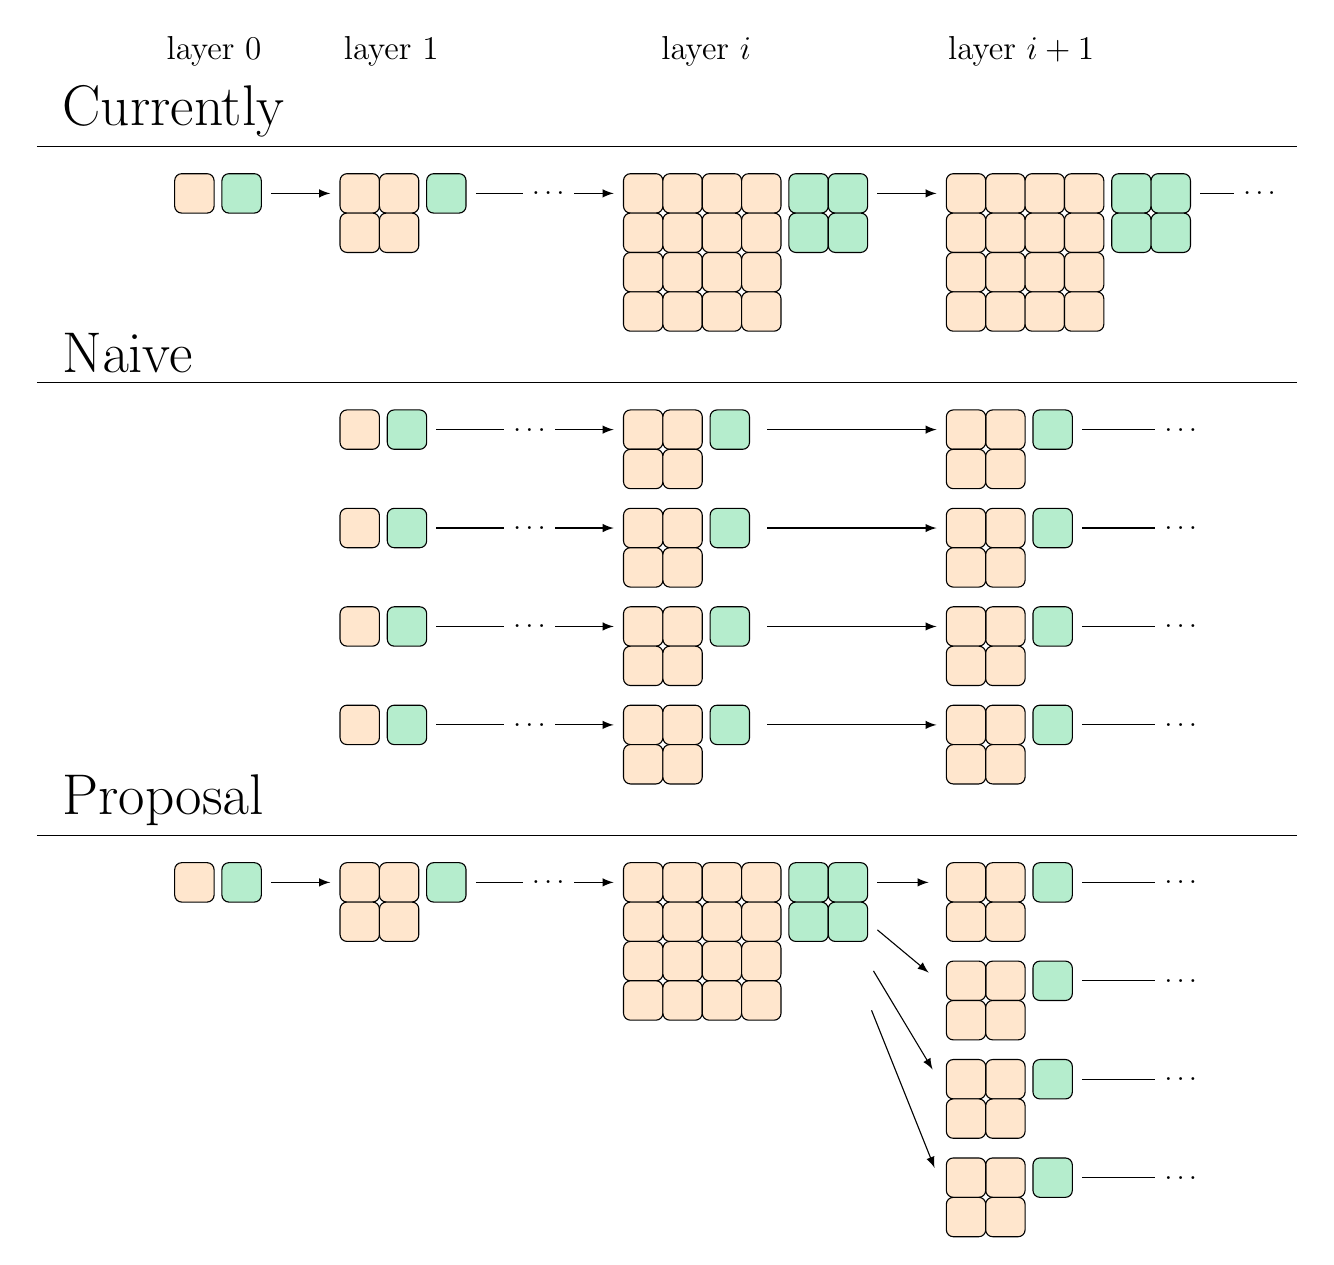
\begin{tikzpicture}
     \node at (0.5cm * 0 + 0.1cm * 0, 0) (H) [array_element, fill=LightColor] {};
     \node at (0.5cm * 1 + 0.1cm * 1, 0) (H) [array_element, fill=tile2] {};

     \node at (0.5cm * 1 + 0.1cm * 1 + 1.5cm * 1, 0) (H) [array_element, fill=LightColor] {};
     \node at (0.5cm * 2 + 0.1cm * 1 + 1.5cm * 1, 0) (H) [array_element, fill=LightColor] {};
     \node at (0.5cm * 1 + 0.1cm * 1 + 1.5cm * 1, -0.5cm) (H) [array_element, fill=LightColor] {};
     \node at (0.5cm * 2 + 0.1cm * 1 + 1.5cm * 1, -0.5cm) (H) [array_element, fill=LightColor] {};
     
     \node at (0.5cm * 3 + 0.1cm * 2 + 1.5cm * 1, -0.0cm) (H) [array_element, fill=tile2] {};

    \node at (0.5cm * 1 + 0.1cm * 1 + 0.25cm, -0.cm) (c1) [] {};
    \node at (0.5cm * 1 + 0.1cm * 1 + 1.5cm * 1 - 0.25cm, -0.cm) (c2) [] {};
    \draw[-latex](c1) -- (c2);

    \node at (0.5cm * 3 + 0.1cm * 2 + 1.5cm * 1 + 0.25cm, -0.cm) (c1) [] {};
    \node at (0.5cm * 3 + 0.1cm * 2 + 1.5cm * 1 + 2.5cm - 0.25cm, -0.cm) (c2) [] {};
    \draw[-latex](c1) --node[empty_element, pos=0.525] {$\dots$} (c2);

    \node at (0.5cm * 8 + 0.1cm * 3 + 1.5cm * 1 + 2.5cm + 0.25cm, -0.cm) (c1) [] {};
    \node at (0.5cm * 8 + 0.1cm * 3 + 1.5cm * 2 + 2.5cm - 0.25cm, -0.cm) (c2) [] {};
    \draw[-latex](c1) -- (c2);

    \node at (0.5cm * 16 + 0.1cm * 4 + 1.5cm * 1 + 2.5cm + 0.25cm, -0.cm) (c1) [] {};
    \node at (0.5cm * 16 + 0.1cm * 4 + 1.5cm * 2 + 2.5cm - 0.25cm, -0.cm) (c2) [] {};
    \draw[-](c1) --node[empty_element, pos=1] {$\dots$} (c2);



    \foreach \la in {0,...,3} {
        \foreach \lb in {0,...,3} {
            \node at (0.5cm * \la + 0.5cm * 3 + 0.1cm * 2 + 1.5cm * 1 + 2.5cm, -0.5cm * \lb) (H\la\lb) [array_element, fill=LightColor] {};
        }
    }
    \foreach \la in {0,...,1} {
        \foreach \lb in {0,...,1} {
            \node at (0.5cm * \la + 0.5cm * 7 + 0.1cm * 3 + 1.5cm * 1 + 2.5cm , -0.5cm * \lb) (H\la\lb) [array_element, fill=tile2] {};
        }
    }

    \foreach \la in {0,...,3} {
        \foreach \lb in {0,...,3} {
            \node at (0.5cm * \la + 0.5cm * 8 + 0.1cm * 3 + 1.5cm * 2 + 2.5cm, -0.5cm * \lb) (H\la\lb) [array_element, fill=LightColor] {};
        }
    }
    \foreach \la in {0,...,1} {
        \foreach \lb in {0,...,1} {
            \node at (0.5cm * \la + 0.5cm * 12 + 0.1cm * 4 + 1.5cm * 2 + 2.5cm , -0.5cm * \lb) (H\la\lb) [array_element, fill=tile2] {};
        }
    }



      \foreach \la in {0,...,3} {
        \node at (0.5cm * 2 + 0.1cm * 1 + 1.0cm, -3cm - 1.25cm * \la) (H) [array_element, fill=LightColor] {};
        \node at (0.5cm * 3 + 0.1cm * 2 + 1.0cm, -3cm - 1.25cm * \la) (H) [array_element, fill=tile2] {};
        
             \node at (0.5cm * 0 + 0.1cm * 2 + 1.5cm * 2 + 2.5cm, -3cm -1.25cm * \la) (H) [array_element, fill=LightColor] {};
     \node at (0.5cm * 1 + 0.1cm * 2 + 1.5cm * 2  + 2.5cm, -3cm -1.25cm * \la) (H) [array_element, fill=LightColor] {};
     \node at (0.5cm * 0 + 0.1cm * 2 + 1.5cm * 2 + 2.5cm, -0.5cm -3cm -1.25cm * \la) (H) [array_element, fill=LightColor] {};
     \node at (0.5cm * 1 + 0.1cm * 2 + 1.5cm * 2 + 2.5cm, -0.5cm - 3cm -1.25cm * \la) (H) [array_element, fill=LightColor] {};
     \node at (0.5cm * 2 + 0.1cm * 3 + 1.5cm * 2 + 2.5cm, -0.0cm - 3cm -1.25cm * \la) (H) [array_element, fill=tile2] {};
     
         \node at (0.5cm * 2 + 0.1cm * 2 + 1.5cm * 1 + 0.25cm, -0.cm - 3cm -1.25cm * \la) (c1) [] {};
    \node at (0.5cm * 3 + 0.1cm * 2 + 1.5cm * 1 + 2.5cm - 0.25cm, -0.0cm - 3cm -1.25cm * \la) (c2) [] {};
    \draw[-latex](c1) --node[empty_element, pos=0.525] {$\dots$} (c2);

     \node at (0.5cm * 6 + 0.1cm * 3 + 1.5cm * 3 + 2.5cm, -3cm -1.25cm * \la) (H) [array_element, fill=LightColor] {};
     \node at (0.5cm * 5 + 0.1cm * 3 + 1.5cm * 3  + 2.5cm, -3cm -1.25cm * \la) (H) [array_element, fill=LightColor] {};
     \node at (0.5cm * 5 + 0.1cm * 3 + 1.5cm * 3 + 2.5cm, -0.5cm -3cm -1.25cm * \la) (H) [array_element, fill=LightColor] {};
     \node at (0.5cm * 6 + 0.1cm * 3 + 1.5cm * 3 + 2.5cm, -0.5cm - 3cm -1.25cm * \la) (H) [array_element, fill=LightColor] {};
     \node at (0.5cm * 7 + 0.1cm * 4 + 1.5cm * 3 + 2.5cm, -0.0cm - 3cm -1.25cm * \la) (H) [array_element, fill=tile2] {};

    \node at (0.5cm * 2 + 0.1cm * 4 + 1.5cm * 2 + 2.5cm + 0.25cm, -0.cm -3cm -1.25cm * \la) (c1) [] {};
    \node at (0.5cm * 5 + 0.1cm * 3 + 1.5cm * 3 + 2.5cm - 0.25cm, -0.cm-3cm -1.25cm * \la) (c2) [] {};
    \draw[-latex](c1) -- (c2);

    \node at (0.5cm * 16 + 0.1cm * 4 + 1.5cm * 1 + 2.5cm + 0.25cm - 1.5cm, -3cm -1.25cm * \la) (c1) [] {};
    \node at (0.5cm * 16 + 0.1cm * 4 + 1.5cm * 2 + 2.5cm - 0.25cm - 1cm, -3cm -1.25cm * \la) (c2) [] {};
    \draw[-](c1) --node[empty_element, pos=1] {$\dots$} (c2);
      }

     \node at (0.5cm * 0 + 0.1cm * 0, 0 - 8.75cm) (H) [array_element, fill=LightColor] {};
     \node at (0.5cm * 1 + 0.1cm * 1, 0- 8.75cm) (H) [array_element, fill=tile2] {};

     \node at (0.5cm * 1 + 0.1cm * 1 + 1.5cm * 1, 0- 8.75cm) (H) [array_element, fill=LightColor] {};
     \node at (0.5cm * 2 + 0.1cm * 1 + 1.5cm * 1, 0 - 8.75cm) (H) [array_element, fill=LightColor] {};
     \node at (0.5cm * 1 + 0.1cm * 1 + 1.5cm * 1, -0.5cm - 8.75cm) (H) [array_element, fill=LightColor] {};
     \node at (0.5cm * 2 + 0.1cm * 1 + 1.5cm * 1, -0.5cm - 8.75cm) (H) [array_element, fill=LightColor] {};
     
     \node at (0.5cm * 3 + 0.1cm * 2 + 1.5cm * 1, -0.0cm - 8.75cm) (H) [array_element, fill=tile2] {};

    \node at (0.5cm * 1 + 0.1cm * 1 + 0.25cm, -0.cm - 8.75cm) (c1) [] {};
    \node at (0.5cm * 1 + 0.1cm * 1 + 1.5cm * 1 - 0.25cm, -0.cm - 8.75cm) (c2) [] {};
    \draw[-latex](c1) -- (c2);

    \node at (0.5cm * 3 + 0.1cm * 2 + 1.5cm * 1 + 0.25cm, -0.cm - 8.75cm) (c1) [] {};
    \node at (0.5cm * 3 + 0.1cm * 2 + 1.5cm * 1 + 2.5cm - 0.25cm, -0.cm - 8.75cm) (c2) [] {};
    \draw[-latex](c1) --node[empty_element, pos=0.525] {$\dots$} (c2);

    \node at (0.5cm * 8 + 0.1cm * 3 + 1.5cm * 1 + 2.5cm + 0.25cm, -0.cm - 8.75cm) (c1) [] {};
    \node at (0.5cm * 8 + 0.1cm * 3 + 1.5cm * 2 + 2.5cm - 0.35cm, -0.cm - 8.75cm) (c2) [] {};
    \draw[-latex](c1) -- (c2);
    
        \node at (0.5cm * 8 + 0.1cm * 3 + 1.5cm * 1 + 2.5cm + 0.25cm, -0.cm - 8.75cm - 0.5cm) (c1) [] {};
    \node at (0.5cm * 8 + 0.1cm * 3 + 1.5cm * 2 + 2.5cm - 0.35cm, -0.cm - 8.75cm - 1.25 cm) (c2) [] {};
    \draw[-latex](c1) -- (c2);

        \node at (0.5cm * 8 + 0.1cm * 3 + 1.5cm * 1 + 2.5cm + 0.25cm, -0.cm - 8.75cm  - 0.5cm * 2) (c1) [] {};
    \node at (0.5cm * 8 + 0.1cm * 3 + 1.5cm * 2 + 2.5cm - 0.35cm, -0.cm - 8.75cm - 1.25 cm * 2) (c2) [] {};
    \draw[-latex](c1) -- (c2);

        \node at (0.5cm * 8 + 0.1cm * 3 + 1.5cm * 1 + 2.5cm + 0.25cm, -0.cm - 8.75cm - 0.5cm * 3) (c1) [] {};
    \node at (0.5cm * 8 + 0.1cm * 3 + 1.5cm * 2 + 2.5cm - 0.35cm, -0.cm - 8.75cm - 1.25 cm * 3) (c2) [] {};
    \draw[-latex](c1) -- (c2);


        \foreach \la in {0,...,3} {
        \foreach \lb in {0,...,3} {
            \node at (0.5cm * \la + 0.5cm * 3 + 0.1cm * 2 + 1.5cm * 1 + 2.5cm, -0.5cm * \lb - 8.75cm) (H\la\lb) [array_element, fill=LightColor] {};
        }
    }
    \foreach \la in {0,...,1} {
        \foreach \lb in {0,...,1} {
            \node at (0.5cm * \la + 0.5cm * 7 + 0.1cm * 3 + 1.5cm * 1 + 2.5cm , -0.5cm * \lb - 8.75cm) (H\la\lb) [array_element, fill=tile2] {};
        }
    }
    \foreach \la in {0,...,3} {
         \node at (0.5cm * 6 + 0.1cm * 3 + 1.5cm * 3 + 2.5cm, -3cm -1.25cm * \la - 5.75cm) (H) [array_element, fill=LightColor] {};
     \node at (0.5cm * 5 + 0.1cm * 3 + 1.5cm * 3  + 2.5cm, -3cm -1.25cm * \la - 5.75cm) (H) [array_element, fill=LightColor] {};
     \node at (0.5cm * 5 + 0.1cm * 3 + 1.5cm * 3 + 2.5cm, -0.5cm -3cm -1.25cm * \la - 5.75cm) (H) [array_element, fill=LightColor] {};
     \node at (0.5cm * 6 + 0.1cm * 3 + 1.5cm * 3 + 2.5cm, -0.5cm - 3cm -1.25cm * \la - 5.75cm) (H) [array_element, fill=LightColor] {};
     \node at (0.5cm * 7 + 0.1cm * 4 + 1.5cm * 3 + 2.5cm, -0.0cm - 3cm -1.25cm * \la - 5.75cm) (H) [array_element, fill=tile2] {};
    \node at (0.5cm * 16 + 0.1cm * 4 + 1.5cm * 1 + 2.5cm + 0.25cm - 1.5cm, -3cm -1.25cm * \la - 5.75cm) (c1) [] {};
    \node at (0.5cm * 16 + 0.1cm * 4 + 1.5cm * 2 + 2.5cm - 0.25cm - 1cm, -3cm -1.25cm * \la - 5.75cm) (c2) [] {};
    \draw[-](c1) --node[empty_element, pos=1] {$\dots$} (c2);




    }
    \node at (-2.0cm, 0.6cm) (line-1-l) {};
    \node at (14cm, 0.6cm) (line-1-r) {};
    \draw[-, thin] (line-1-l.center) -- (line-1-r.center) node[pos=0.0125, above right] {\huge Currently};
    
    \node at (-2.0cm, 0.6cm - 3cm) (line-1-l) {};
    \node at (14cm, 0.6cm - 3cm) (line-1-r) {};
    \draw[-, thin] (line-1-l.center) -- (line-1-r.center) node[pos=0.0125, above right] {\huge Naive};
    
\node at (-2.0cm, 0.6cm - 5cm - 3 * 1.25cm) (line-1-l) {};
\node at (14cm, 0.6cm - 5cm - 3 * 1.25cm) (line-1-r) {};
    \draw[-, thin] (line-1-l.center) -- (line-1-r.center) node[pos=0.0125, above right] {\huge Proposal};

\node at (0.25cm, 1.8cm) (laag0) {\large layer $0$};
\node at (0.25cm + 2.25cm, 1.8cm) (laag0) {\large layer $1$};
\node at (0.25cm + 6.25cm, 1.8cm) (laag0) {\large layer $i$};
\node at (0.25cm + 10.25cm, 1.8cm) (laag0) {\large layer $i + 1$};

\end{tikzpicture}
\end{adjustbox}
  \caption{Subdivision strategy deeper layers of the linkless octree.}
  \label{fig:vo-textures}
\end{figure}
